\section{Interaction Trace and Failure Case}
\label{app:trace}

Figure~\ref{fig:workflow} follows two requests from the frozen evaluation through the pipeline; the candidates are recorded outputs and the validator verdicts are recomputed with the deterministic validator.
Figure~\ref{fig:failure} shows the screenshot of an accepted but unfaithful output (\S\ref{sec:eval}, failure~i).

\begin{figure*}[t]
\centering
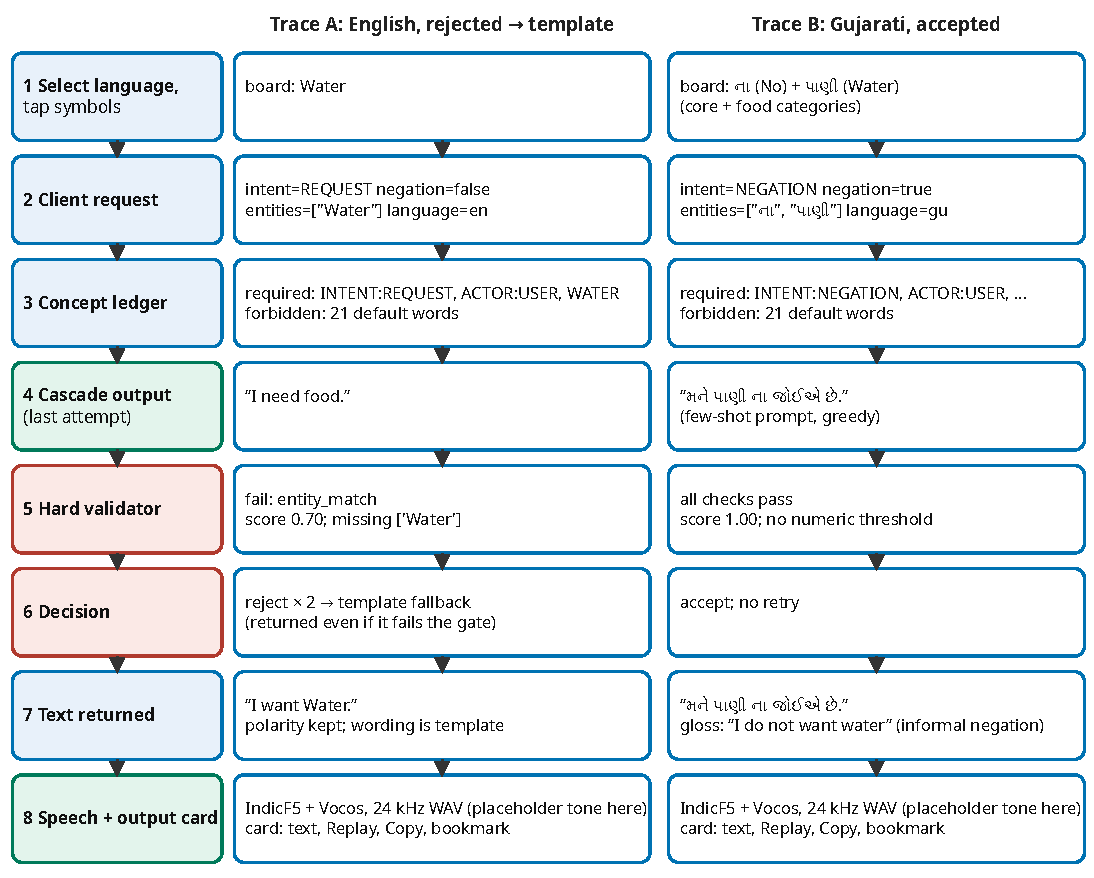
\includegraphics[width=0.86\textwidth]{figures/workflow.pdf}
\caption{Interaction flow for an English request (cascade output rejected twice, template returned) and a Gujarati request (cascade output accepted). English gloss of Trace~B: ``I do not want water'' (informal negation; not native-reviewed).}
\label{fig:workflow}
\end{figure*}

\begin{figure}[t]
\centering
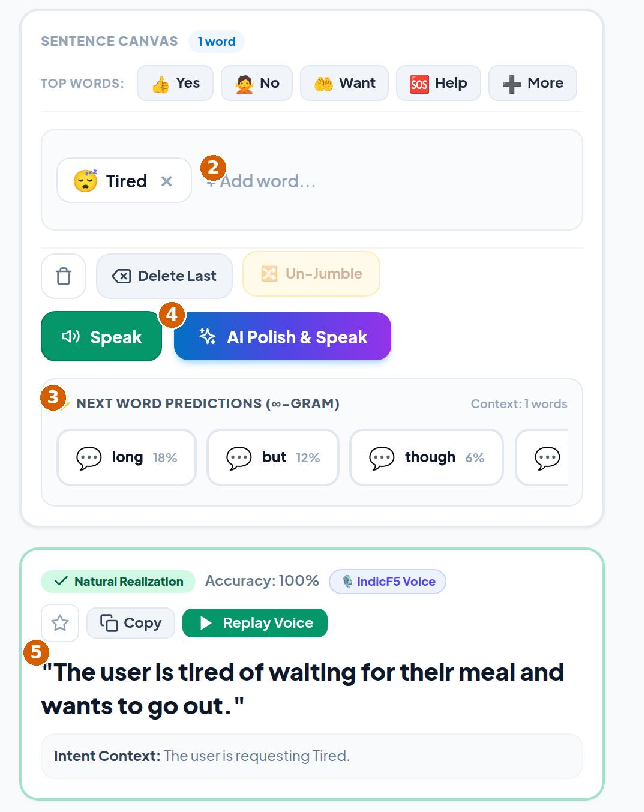
\includegraphics[width=0.72\columnwidth]{figures/ui_failure.pdf}
\caption{English, \emph{Tired}: the client sends \textsc{request}; the gate accepts a fluent sentence that adds unselected content. The card shows ``Accuracy: 100\%''. This screenshot is a different sample from the evaluated one. Callouts as in Figure~\ref{fig:ui}.}
\label{fig:failure}
\end{figure}

\section{Scorer Definitions}
\label{app:scorer}
Retention is the share of required concept instances present (lexicon forms with inflection stems). Polarity is correct when a negator is present exactly if the gold message is negated. The act is correct when a request marker (want, need, \hi{चाहिए}, \gu{જોઈએ}, \hi{हवे}) or, for feelings, a feeling marker without a request marker is present. A concept is \emph{added} if any other board concept or a time, meal or venue word occurs. An output is \emph{off-task} if it is a refusal, a third-person report (``the user\ldots''), empty, longer than 25 tokens, or contains Latin text in an Indic target. Scenarios, lexicon, scorer and raw outputs are in \texttt{eval/}.

\section{Refiner Fine-Tuning and Results}
\label{app:refiner}
The English refiner fine-tunes \texttt{google/flan-t5-small} (revision \texttt{0fc9ddf}, 76,961,152 parameters) to map selected concepts and a user intent to one sentence (Table~\ref{tab:refiner}). Training used fp32 with learning rate $10^{-4}$, weight decay 0.01, batch size 16 with two accumulation steps, 10 epochs (960 updates), source and target limits of 256 and 64 tokens, seed 42, and one NVIDIA TITAN Xp (204\,s, 2.4\,GiB peak); the checkpoint with the lowest validation loss is kept. The fluency arm first adapts for 500 updates on 4,380 denoising pairs. Training, validation and test hold 3,052, 384 and 384 template-generated payloads in 318, 40 and 40 disjoint groups. Because references come from the same template families as the rule path, rule and hybrid scores are exact by construction; the model scores are the informative ones.

\begin{table}[t]
\centering\footnotesize
\setlength{\tabcolsep}{3pt}
\begin{tabular}{@{}lcc@{}}
\toprule
Test (384 payloads) & AAC only & Fluency, then AAC \\
\midrule
Raw selection & \RefARaw{} & \RefFRaw{} \\
Rules & \RefARules{} & \RefFRules{} \\
Fine-tuned model & \RefAModel{} & \RefFModel{} \\
Hybrid (rules + model) & \RefAHybrid{} & \RefFHybrid{} \\
Negation errors (not raw) & 0/172 & 0/172 \\
Model latency, median (ms) & \RefALat{} & \RefFLat{} \\
\bottomrule
\end{tabular}
\caption{Exact match of the refiner, recomputed from the raw predictions of the training kit (it equals the kit's own \texttt{metrics.csv}). The model weights are not in the package; the configuration and tokenizer are.}
\label{tab:refiner}
\end{table}
